\section{Diagrammes de s�quence}


\subsection{Ajout d'un noeud}

Le diagramme suivant montre la s�quence de l'ajout d'un noeud � la simulation.

\begin{figure}[H]
	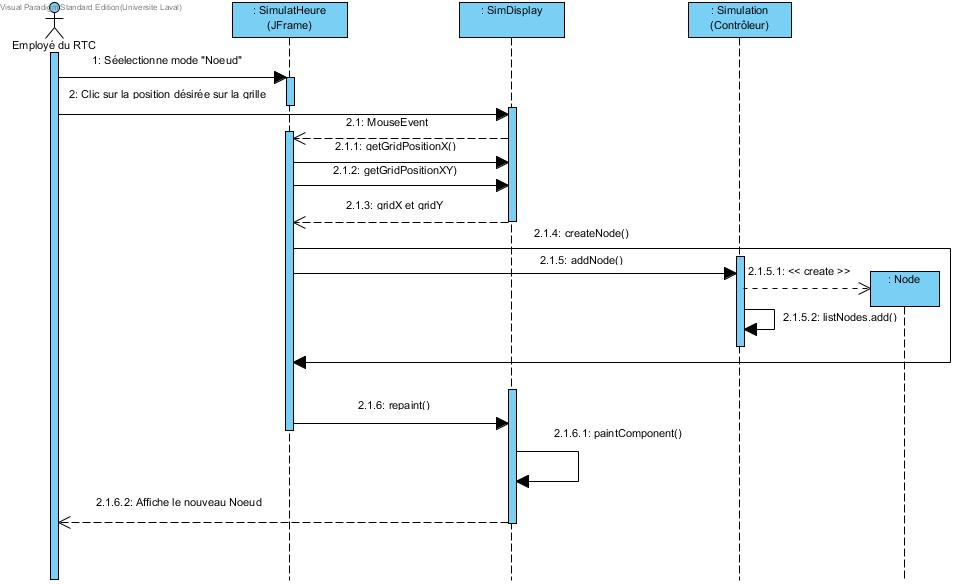
\includegraphics[scale=0.4]{fig/DSS/AddNode.jpg}
	\centering
	\caption{Diagramme de s�quence: ajout d'un noeud}
	\label{f:dss_addNode}
\end{figure}

\subsection{Ajout d'une ar�te}

Le diagramme suivant montre la s�quence de l'ajout dun objet Line � la simulation � partir d'un deux points (Node) non-existants.

\begin{figure}[H]
	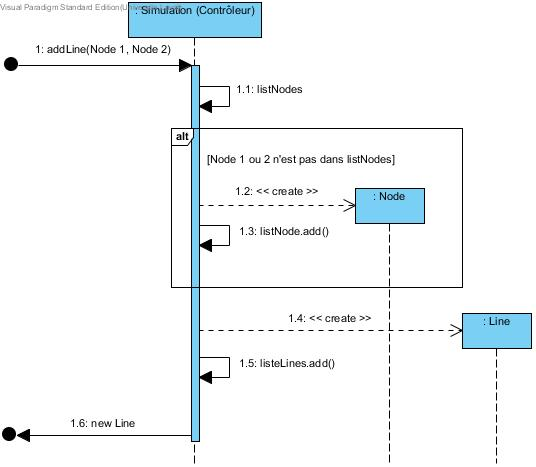
\includegraphics[scale=0.7]{fig/DSS/AddLine.jpg}
	\centering
	\caption{Diagramme de s�quence: ajout d'une ar�te}
	\label{f:dss_addLine}
\end{figure}

\subsection{Simuler}

Le diagramme suivant montre la s�quence du processus de d�marrage d'une simulation par l'usager.

\begin{figure}[H]
	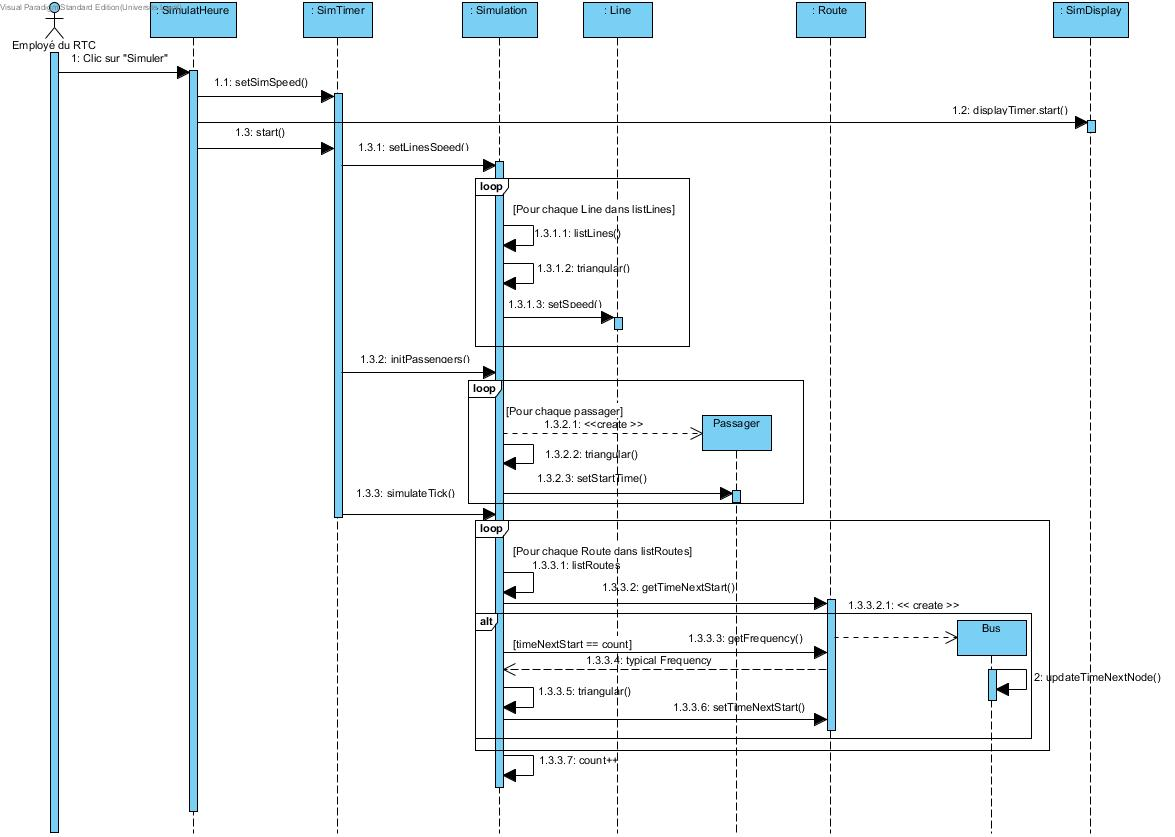
\includegraphics[scale=0.3]{fig/DSS/Simulation.jpg}
	\centering
	\caption{Diagramme de s�quence: d�marrage d'une simulation}
	\label{f:dss_addLine}
\end{figure}

\subsection{Distribution triangulaire}

Le diagramme suivant montre comment la fonction triangular() est utilis� afin de d�terminer la vitesse d'un segment.

\begin{figure}[H]
	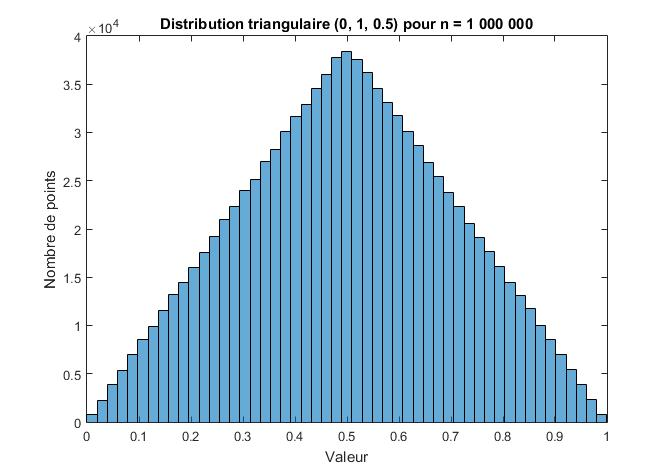
\includegraphics[scale=0.8]{fig/DSS/triangular.jpg}
	\centering
	\caption{Diagramme de s�quence: distribution triangulaire de l'assignation de la vitesse � un segment}
	\label{f:dss_triangular}
\end{figure}

\subsection{Position d'un autobus}

Le diagramme suivant montre comment r�cup�rer la position d'un autobus.

\begin{figure}[H]
	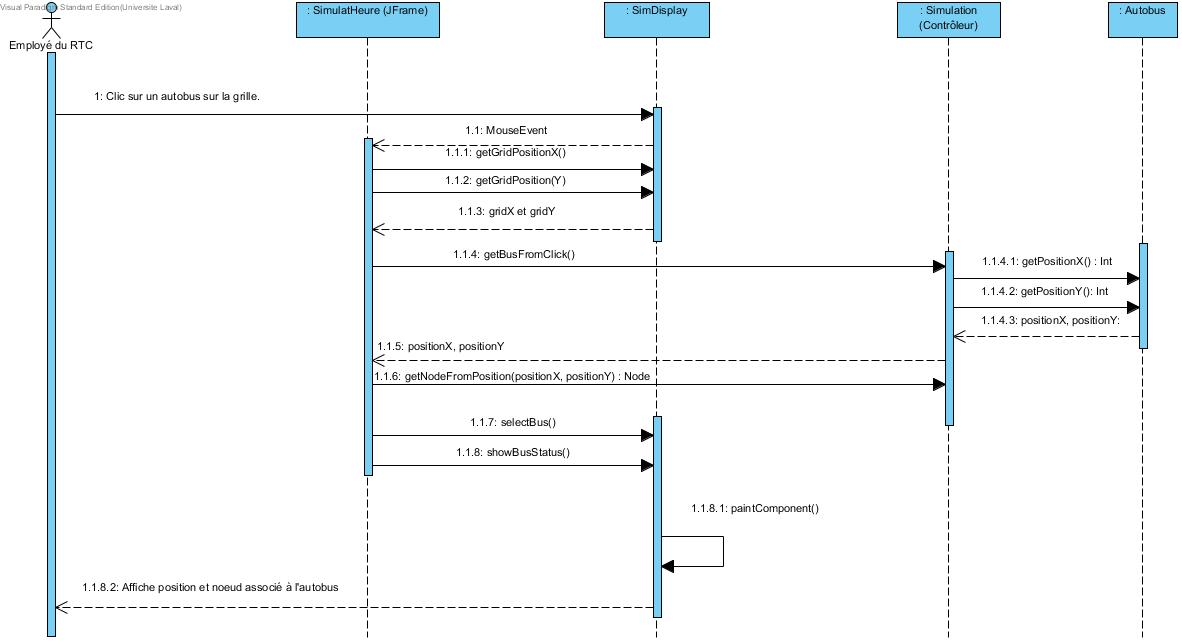
\includegraphics[scale=0.4]{fig/DSS/positionBus.jpg}
	\centering
	\caption{Diagramme de s�quence: Position d'un autobus}
	\label{f:dss_bus}
\end{figure}
